\documentclass[]{article}

% Imported Packages
%------------------------------------------------------------------------------
\usepackage{amssymb}
\usepackage{amstext}
\usepackage{amsthm}
\usepackage{amsmath}
\usepackage{enumerate}
\usepackage{fancyhdr}
\usepackage[margin=1in]{geometry}
\usepackage{graphicx}
%\usepackage{extarrows}
%\usepackage{setspace}
%\usepackage{xcolor}
\usepackage{color}
\usepackage{multirow} 
%------------------------------------------------------------------------------

% Header and Footer
%------------------------------------------------------------------------------
\pagestyle{plain}  
\renewcommand\headrulewidth{0.4pt}                                      
\renewcommand\footrulewidth{0.4pt}                                    
%------------------------------------------------------------------------------

% Title Details
%------------------------------------------------------------------------------
\title{Deliverable \#1: Software Requirement Specification (SRS)}
\author{SE 3A04: Software Design II -- Large System Design}
\date{Febuary 16, 2023}
                            
%------------------------------------------------------------------------------

% Document
%------------------------------------------------------------------------------
\begin{document}

\maketitle	
\noindent{\bf Tutorial Number:} T02\\
{\bf Group Number:} G6 \\
{\bf Group Members:} 
\begin{itemize}
	\item Emily Perica
	\item Harman Bassi
    \item Kyen So
    \item Kelly Deng
    \item Swesan Pathmanathan 
\end{itemize}

\section*{IMPORTANT NOTES}
\begin{itemize}
	\item Be sure to include all sections of the template in your document regardless whether you have something to write for each or not
	\begin{itemize}
		\item If you do not have anything to write in a section, indicate this by the \emph{N/A}, \emph{void}, \emph{none}, etc.
	\end{itemize}
	\item Uniquely number each of your requirements for easy identification and cross-referencing
	\item Highlight terms that are defined in Section~1.3 (\textbf{Definitions, Acronyms, and Abbreviations}) with \textbf{bold}, \emph{italic} or \underline{underline}
	\item For Deliverable 1, please highlight, in some fashion, all (you may have more than one) creative and innovative features. Your creative and innovative features will generally be described in Section~2.2 (\textbf{Product Functions}), but it will depend on the type of creative or innovative features you are including.
\end{itemize}

\newpage
\section{Introduction}
\label{sec:introduction}
% Begin Section

\hspace{5mm}This SRS describes the software requirements for our messaging application, MacMessenger. The application is meant to provide a secure means of communication within a company. This document will outline the purpose, project scope, requirements, and use cases of the product. \\


\subsection{Purpose}
\label{sub:purpose}
% Begin SubSection
\hspace{5mm}This SRS is meant to provide an overview of the requirements imposed upon the MacMessenger system, providing information on functional and non-functional requirements, as well as use cases and potential employee characteristics. The intended audience of this SRS is all stakeholders involved in the MacMessenger product. It will provide a high-level overview of the requirements needed to begin designing the product, using a non-technical language that may be understood by stakeholders who may have a broad range in their understanding of technical terms.


% End SubSection

\subsection{Scope}
\label{sub:scope}
% Begin SubSection
\hspace{5mm}MacMessenger is a secure messaging application that allows employee to send messages on company issued Android devices through sessions of key authentications and store chat logs on the server. It also allows employee to create group chats, attaching files and customizing account. 

\hspace{5mm}Employees are required to sign-in or create an account to access the application. Main services of the application include “Sending messages”, “Creating group chat”, “Attaching files” and “Customizing account”. In “Sending messages”, employee will fetch a key from KDC and authenticates with the server to start a session and send messages. System will encrypt/decrypt the message using symmetric key cryptography and store the chat log onto the server. In “Creating group chat”, employee(s) can add contacts to group chat creation and others will receive notification for being added. In “Attaching files”, an employee can add a file by dragging it into chat box and click “Send” to display it in chat interface. In “Customizing account”, an employee can modify their account information such as avatar, nick names etc.

\hspace{5mm}The objective of this application is to avoid corporate espionage within the organization by establishing secure communication via authentication keys on company android devices, so to reduce the risks of information leakage and cybersecurity attack. As the software will be used by employees who may have minimal technical background, the software will be intuitive to navigate and accessible. The software will also have fast response time since it is for business use. 

\hspace{5mm}The goal of this software is to promote safe communication means between employees, as companies heavily rely on online communications nowadays. 

% End SubSection

\subsection{Definitions, Acronyms, and Abbreviations}
\label{sub:definitions_acronyms_and_abbreviations}
% Begin SubSection
\textbf{DoS}: Denial of Service attack. A type of cyberattack in which the attacker attempts to stall services by flooding the server with requests.\vspace{2mm}\\
\textbf{Employee}: A worker employed by the company utilizing MacMessenger. Used interchangeably with ‘user’ throughout the SRS.\vspace{2mm}\\
\textbf{KDC}: Key Distribution Center. Used to generate all keys used in a secure communication session.\vspace{2mm}\\
\textbf{MacMessenger}: Secure messaging application.\vspace{2mm}\\
\textbf{Symmetric-key cryptosystem}: An encryption scheme in which both involved parties have access to a private, pre-determined key.\\

% End SubSection

\subsection{References}
\label{sub:references}
% Begin SubSection
\begin{thebibliography}{9}
    \bibitem{lamport94}
    Gillis, A. (2022, June). What is a security audit? TechTarget. https://www.techtarget.com/searchcio/definition/security-audit
    \bibitem{lamport94}
    Make Google Messages more accessible - Google Messages. (n.d.). Support.google.com. https://support.google.com/messages/answer/6105764?hl=en 
    \bibitem{lamport94}
    Non-functional Requirements: Examples, Types, How to Approach. (2022, July 26). AltexSoft. https://www.altexsoft.com/blog/non-functional-requirements/
    \bibitem{lamport94}
    Understanding SOLID Principles and Clean Architecture. (n.d.). Www.yourteaminindia.com. Retrieved February 18, 2024, from https://www.yourteaminindia.com/blog/understanding-solid-principles-and-clean-architecture#:~:text=Architecture 
    \bibitem{lamport94}
    NIST. (2022, July 21). NIST Cybersecurity & Privacy Program [Review of NIST Cybersecurity & Privacy Program].https://www.nist.gov/system/files/documents/2022/07/21/Extended%20Cybersecurity%20Vitals%20Fact%20Sheet.pdf 
    \bibitem{lamport94}
    frank@v51.com. (2019). Your privacy rights - IPC. IPC. https://www.ipc.on.ca/privacy-individuals/your-privacy-rights/ 
    \bibitem{lamport94}
    Wang, Y., Huang, Y., Li, J., & Zhang, J. (2021). The effect of mobile applications’ initial loading pages on users’ mental state and behavior. Displays, 68, 102007. https://doi.org/10.1016/j.displa.2021.102007 
    \bibitem{lamport94}
    Android OS. (n.d.). Endoflife.date. https://endoflife.date/android 
    \bibitem{lamport94}
    Core app quality. (n.d.). Android Developers. https://developer.android.com/docs/quality-guidelines/core-app-quality
\end{thebibliography}
% End SubSection

\subsection{Overview}
\label{sub:overview}
% Begin SubSection
\hspace{10mm}Section 2 provides a general description of the product, delving into the perspectives, functions, users, constraints, and assumptions that must be considered when designing the system. Section 3 presents a Use Case Diagram to provide the reader with a visual understanding of the desired flow of the system. Section 4 describes the Functional Requirements of the system, and section 5 describes the Non-Functional Requirements of the system. Lastly, Section A contains the Division of Labour of this SRS.
% End SubSection

% End Section

\section{Overall Product Description}
\label{sec:overall_description}
% Begin Section

\subsection{Product Perspective}
\label{sub:product_perspective}
% Begin SubSection
\hspace{5mm}Compared to applications like WhatsApp and Singal the main property of the MacMessenger will be to provide proper security between the employees of the company. The end-to-end encryption ensures that the messages in the application are not easily attainable like Signal. MacMessenger focuses on providing a key that would be used to ensure encryption like Signal. Signal makes sure that the key is also not stored in external servers to ensure discrepancy. In terms of looks, the application would resemble Facebook Messenger as it provides the user with a very intuitive design making it easy to understand how to use the messenger app. MacMessenger also allows the user to add or remove people from chat groups. This would resemble all the previous related apps mentioned.
\newline
\newline
\indent The application itself is self-contained as all the main applications are within the company. The product communicates with the businesses database to ensure the employees have an account for specific authorization. Overall, it depends on existing interfaces that exist within the company to complete authorization and beyond that everything else is done within the MacMessenger ecosystem. This is to ensure secrecy and protect valuable data.
\newline
\newline
\textbf{Interfaces within the Overall System:}
\newline
\newline
\indent The User Interface is an important aspect when it comes to what the employee sees and interacts with. The employee is presented with the front-end and is allowed to interact with it, given the certain perameters of the application. This would be the system that takes in the user inputs to provide wanted results.
\newline
\newline
\indent The Messaging System is where the encryption and overall distribution of messages occurs. When the employee sends their message it enters the system, encrypted it and then sends it to the other user. The system is also responsible for communicating with the other systems to ensure the authorization of the user and the proper distribution of keys.
\newline
\newline
\indent Authentication Server is where the system would connect to the business’s database to ensure that the employee is entering their correct information and if they are allowed access to the application. This entity would communicate with the Messaging System to authenticate the user.
\newline
\newline
\indent The KDC Server is responsible for providing and storing the keys that would be sent to the employee. This is to ensure it helps encrypt the messages sent by the user. This will regularly be updating itself to ensure that users will always be provided with new keys to ensure security.
\newline
\newline
\indent The Chat Log Database will store all the chat logs from the application. After each message is sent it is stored within the chat log database so that an authorized person has access to it when need be. This is to ensure that every chat can be accessed even after chat deletion to ensure a proper record of every company discussion within the application.
\newline
\begin{center}
    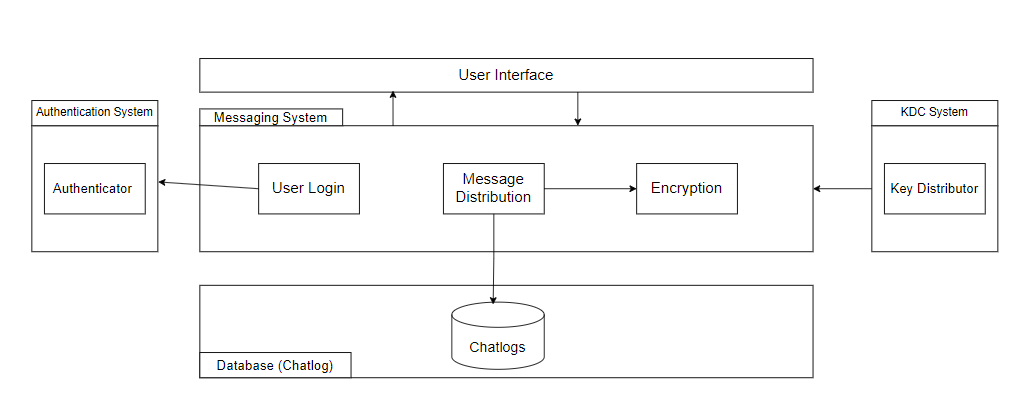
\includegraphics{Graphics/blockdiagram.png}\\
    \emph{Figure 1: Block diagram for different systems involved}
\end{center}
% End SubSection

\subsection{Product Functions}
\label{sub:product_functions}
% Begin SubSection
\hspace{5mm}The software will ensure secure connection and communication between employees by generating a key only for those who are authorized using a mediated authentication protocol. The key is generated and contained within a KDC server which frequently updates the authorized communicating agents’ keys. Messages between communicating agents will be encrypted and decrypted using a symmetric-key crypto-system and stored securely on the server, including complete chat logs, communicating agent identifiers and date/time. 
\newline
\newline
\textbf{Security:}
\begin{itemize}
\item Access to the chat application is verified by an authentication process which authorizes each employee individually 
\item Every employee’s access to the chat application is controlled by a server that gives access only to those authorized in the form of a key  
\item The server will frequently update and ensure that each registered employee is connected securely by providing a new key 
\item The application will encrypt every outgoing message and decrypts every incoming message using an algorithm 
\end{itemize}
\textbf{Database:}   
\begin{itemize}
\item Detailed information including an accurate chat log along with the identifier of the employees and the messages’ time and date will be securely stored. 
\item All attached files that are sent will be securely stored 
\end{itemize}
\textbf{User Interaction:}  
\begin{itemize}
\item Employees can create and communicate in group chats for secure communication between departments or teams. 
\item Employees can securely reset their password through the company provided email to regain access to their account 
\item Employees can send and receive files while the application will encrypt outgoing files and decrypt incoming files 
\item Employees can customize their account by changing their nickname, profile photo and password. 
\end{itemize}
\begin{center}
    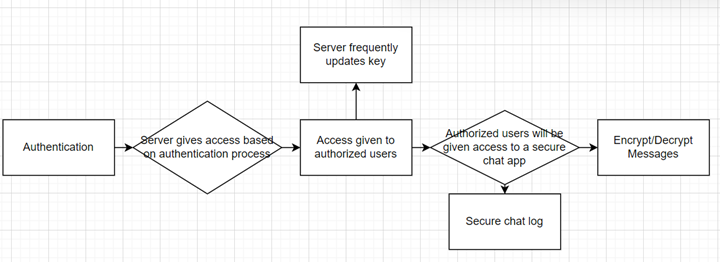
\includegraphics{Graphics/2.2diagram.png}\\
    \emph{Figure 1: Functions and Relationships}
\end{center}

% End SubSection

\subsection{User Characteristics}
\label{sub:user_characteristics}
% Begin SubSection
This system is meant to be user friendly and simple to navigate; it will be designed with the following stakeholders in mind:\\
User group 1: Interns (Primary stakeholder)
\begin{itemize}
    \item Part-way through a bachelor’s degree
    \item 19-23 years old
    \item Android users
    \item Have internet access.
    \item Little to no experience in their field
\end{itemize}

\noindent User group 2: Full time employees (Primary stakeholder)
\begin{itemize}
    \item Minimum education: bachelor’s degree
    \item 23+ years old
    \item Android users
    \item Have internet access.
    \item Experience ranging from junior level to upper management.
\end{itemize}

\noindent User group 3: IT Employees/Technical Maintainers (Tertiary stakeholder)
\begin{itemize}
    \item Have at least a bachelor’s degree
    \item Tech-savvy
    \item 23+ years old
    \item Have internet access.
    \item Have a thorough understanding of the communication system and its technical maintenance.
\end{itemize}
% End SubSection

\subsection{Constraints}
\label{sub:constraints}
% Begin SubSection
\hspace{5mm}The project's development is bound by several key constraints that affect its timeline, design, and functionality. The necessity to complete the project by a specified due date, alongside the imperative to balance security measures with a employee-friendly design, notably influences the development approach. Compatibility requirements with Android devices, considerations for mobile resource limitations, and the need to ensure the application operates reliably across varied network conditions further restrict development choices. Additionally, adherence to data protection laws and integration with existing organizational infrastructure pose significant considerations.

\hspace{5mm}Furthermore, the application's design must prioritize scalability and ease of maintenance to accommodate future growth, all while adhering to a defined budget. Secure data management, including chat history and compliance with data retention policies, alongside comprehensive testing, and quality assurance processes, are crucial for safeguarding employee information and ensuring the app's reliability. These constraints collectively guide the development process, ensuring the final product meets organizational needs, regulatory requirements, and employee expectations, even within the constraints of cost, performance, and security.

% End SubSection

\subsection{Assumptions and Dependencies}
\label{sub:assumptions_and_dependencies}
% Begin SubSection
\begin{itemize}
	\item The software will only be provided on company-issued Android devices. Not supported on other devices in the market.
    \item Devices will have stable connection to the Internet during communication. 
    \item Assume that only employees within the company will use the software. 
    \item Assume there is no limitation on the number of people in a group chat.  
    \item The software shall function on the latest release of the Android operating system. 
    \item Assume that the key generated in one session can be used for an unlimited number of chats. 
    \item It is assumed that the server for storing chat history logs will be provided, and will always have sufficient storage space for chat logs. 
    \item It is assumed that there is a database for storing existing employee names/passwords
    \item The software will only be used within Canada.

\end{itemize}
% End SubSection

\subsection{Apportioning of Requirements}
\label{sub:apportioning_of_requirements}
% Begin SubSection
\hspace{5mm}Certain requirements may be earmarked for implementation in future versions of the system to ensure that the initial release is manageable, focuses on core functionalities, and can meet the deadline and budget constraints. Advanced features such as enhanced encryption algorithms for even higher security, deeper integration with other organizational systems, additional employee customization options, expanded compatibility with a broader range of Android versions, or more sophisticated chat functionalities (like file attachment or editing messages, group management features) might be deferred. 
% End SubSection

% End Section
\section{Use Case Diagram}
\label{sec:use_case_diagram}
% Begin Section
\begin{center}
    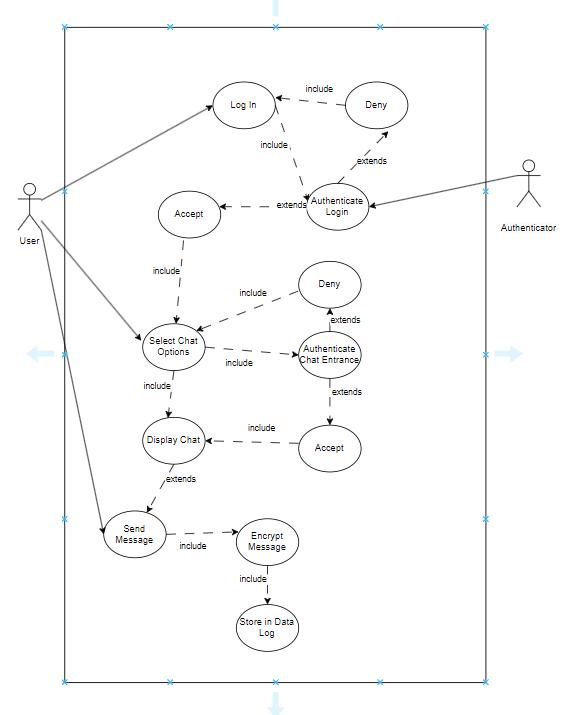
\includegraphics{Graphics/usecaseBetter.png}\\
    \emph{Figure 3: Use Case diagram for Sending a Message}
\end{center}

\hspace{5mm}Sending Message is the business event that the use case diagram represents. The use case diagram is to highlight how the employee would go about sending a secure message through the application. So, the user will login in, then select the chat room and send the message. There are also some secondary scenarios covered like if the login is denied. This is to cover the main possibilities within the sending business events.
% End Section

\section{Highlights of Functional Requirements}
\label{sec:functional_requirements}
% Begin Section
The business events we will consider:

\textbf{BE1.} Sending message

\textbf{BE2.} Group chat creation (Creative Feature)

\textbf{BE3.} Password recovery (Creative Feature)

\textbf{BE4.} Customize account (Creative Feature)

\textbf{BE5.} Logging in

\textbf{BE6.} Account register

\textbf{BE7.} Attaching file (Creative Feature)

\textbf{BE8.} Accessing chatlog

\textbf{BE9.} Updating key\\

\noindent The viewpoints we will consider:

\textbf{VP1.} Employee

\textbf{VP2.} Administrator

\textbf{VP3.} Customer support

\textbf{VP4.} Maintenance

\textbf{VP5.} Cybersecurity

\textbf{VP6.} Management\\

\noindent {\bf Interpretation:} Specify any liberties you took in interpreting business events, if necessary.\\

\begin{enumerate}[{\bf BE1.}]
	\item Sending Message\\
        \textbf{Pre-condition:} The employee must already have an account.
		\begin{enumerate}[{\bf VP1.}]
			\item Employee \\
				\textbf{Main Success Scenario:}
                \begin{enumerate}[{  1.}]
                    \item Employee opens the MacMessenger app on their phone.
                    \item System requires the employee to login and displays the login fields.
                    \item Employee logs into the app.
                    \item System authenticates the employee.
                    \item System shows the account, and chat options.
                    \item Employee chooses chat option. 
                    \item System authenticates employee.
                    \item System displays chat box.
                    \item Employee enters message into chat box and clicks send.
                    \item System encrypts message. 
                    \item System sends message to the recipient.
                    \item Recipient receives encrypted message. 
                    \item System decrypts message with key.
                    \item System stores message in the chatlog.
                \end{enumerate}
                \textbf{Secondary Scenario:}
                \begin{enumerate}
                    \item[4i.] System fails to authenticate the employee in login.
                    \begin{enumerate}
                        \item[4i.1] System prompts for re-entry of login details.
                        \item[4i.2] Sending Message failed.
                    \end{enumerate}
                    \item[7i.] System fails to authenticate the employee for the chat session.
                    \begin{enumerate}
                        \item[7i.1] System logs the employee out.
                        \item[7i.2] Sending Message failed.
                    \end{enumerate}
                    \item[9i.] employee enters an invalid format or restricted content in the message.
                    \begin{enumerate}
                        \item[9i.1] System displays an error message and requests correction.
                        \item[9i.2] Sending Message failed.
                    \end{enumerate}
                    \item[10i.] System fails to encrypt the message.
                    \begin{enumerate}
                        \item[10i.1] System notifies the employee of the encryption error.
                        \item[10i.2] Sending Message failed.
                    \end{enumerate}
                    \item[11i.] System fails to send the message to the recipient.
                    \begin{enumerate}
                        \item[11i.1] System notifies the employee of the sending error.
                        \item[11i.2] Sending Message failed.
                    \end{enumerate}
                    \item[13i.] System fails to decrypt the message for the recipient.
                    \begin{enumerate}
                        \item[13i.1] Recipient receives a notification of decryption error.
                        \item[13i.2] Message is stored encrypted, pending resolution.
                    \end{enumerate}
                \end{enumerate}
		  \item Administrator \\
				N/A
            \item Customer support \\
            \begin{enumerate}
                \item[4i.] System displays an error message to try again or contact customer support for assistance.
                \begin{enumerate}
                    \item[4i.1] System provides a direct link or contact details for the MacMessenger customer support team.
                \end{enumerate}
                \item[9i.] Employee enters an invalid format or restricted content in the message.
                \begin{enumerate}
                    \item[9i.1] System displays an error message and requests correction.
                    \item[9i.2] Sending Message failed.
                \end{enumerate}
                \item[10i.] System fails to encrypt the message.
                \begin{enumerate}
                    \item[10i.1] System notifies the employee of the encryption error.
                    \item[10i.2] Sending Message failed.
                \end{enumerate}
                \item[11i.] System fails to send the message to the recipient.
                \begin{enumerate}
                    \item[11i.1] System notifies the employee of the sending error.
                    \item[11i.2] Sending Message failed.
                \end{enumerate}
            \item Maintenance \\
            N/A
            \item Cybersecurity \\
            N/A
            \item Management \\
            N/A \\
		\end{enumerate}
		{\bf Global Scenario:}\\
        \begin{enumerate}[{  }]
            \item \textbf{Precondition:} The employee must already have an account.
            \item \textbf{Main Success Scenario:}
            \begin{enumerate}[{  1.}]
                \item Employee opens the MacMessenger app on their Android device.
                \item System requires the employee to login and 
            \end{enumerate}
        \end{enumerate}
		\textcolor{red}{Insert Scenario Here}
	\item Business Event Name \#2
	\begin{enumerate}[{\bf VP1.}]
		  \item Viewpoint Name \#1 \\
		  \textcolor{red}{Insert Scenario Here}
		\item Viewpoint Name \#2 \\
		\textcolor{red}{Insert Scenario Here}
	\end{enumerate}
	{\bf Global Scenario:}\\
	\textcolor{red}{Insert Scenario Here}
\end{enumerate}

\begin{enumerate}[{\bf BE4.}]
    \item Customizing Account \\ 
        \textbf{Pre-condition:} The employee must already have an account and the employee is logged in 
        \begin{enumerate}
            \item[VP1.] Employee \\
                \textbf{Main Success Scenario:}
                \begin{enumerate}
                    \item Employee selects “Settings” from main menu. 
                    \item System displays all account information and options that can be customized. 
                    \item Employee customizes account and presses “Save”. 
                    \item System authenticates Employee to approve changes. 
                \end{enumerate}
                \textbf{Secondary Scenario:}
                \begin{enumerate}
                    \item[3i.] Employee has an invalid change
                    \begin{enumerate}
                        \item[3i.1] Employee has an invalid change
                        \item[3i.2] System cannot save changes
                        \item[3i.3] Customizing account failed, return to BE4.VP1.2
                    \end{enumerate}
                    \item[4i.]
                    \begin{enumerate}
                        \item[4i.1] System fails to authenticate Employee
                        \item[4i.2] System cannot save changes
                        \item[4i.3] Customizing account failed, return to BE4.VP1.2
                    \end{enumerate}
                \end{enumerate}
            \item[VP2.] Administrator \\
            \indent N/A 
            \item[VP3.] Customer Support \\
            \indent N/A 
            \item[VP4.] Maintenance \\
            \indent N/A 
            \item[VP5.] Cybersecurity \\
            \indent N/A 
            \item[VP6.] Management \\
            \indent N/A 
        \end{enumerate}
        {\bf Global Scenario:}\\
        \begin{enumerate}
            \item \textbf{Precondition:} The employee must already have an account and the employee is logged in
            \item \textbf{Main Success Scenario:}
            \begin{enumerate}
                \item Employee selects “Settings” from main menu. 
                \item System displays all account information and options that can be customized. 
                \item Employee customizes account and presses “Save”. 
                \item System authenticates Employee to approve changes. 
            \end{enumerate}
            \item \textbf{Secondary Scenario:}
            \begin{enumerate}
                \item[3i.] Employee has an invalid change
                \begin{enumerate}
                    \item[3i.1] Employee has an invalid change
                    \item[3i.2] System cannot save changes
                    \item[3i.3] Customizing account failed, return to BE4.VP1.2
                \end{enumerate}
                \item[4i.]
                \begin{enumerate}
                    \item[4i.1] System fails to authenticate Employee
                    \item[4i.2] System cannot save changes
                    \item[4i.3] Customizing account failed, return to BE4.VP1.2
                \end{enumerate}
            \end{enumerate}
        \end{enumerate}
\end{enumerate}


\begin{enumerate}[{\bf BE5.}]
    \item Logging in \\ 
        \textbf{Pre-condition:} The employee must already have an account. 
        \begin{enumerate}
            \item[VP1.] Employee \\
                \textbf{Main Success Scenario:}
                \begin{enumerate}
                    \item System prompts the employee to enter their login information.  
                    \item Employee enters their login information and presses “Request Key”.  
                    \item System uses a mediated authentication protocol to verify the employee’s information. 
                    \item System generates a key, if authorized, and displays it on screen 
                    \item Employee inputs the correct key and gains access to the application 
                \end{enumerate}
                \textbf{Secondary Scenario:}
                \begin{enumerate}
                    \item[2i.] Incorrect Information
                    \begin{enumerate}
                        \item[2i.1] Incorrect Information
                        \item[2i.2] Login failed, return to BE5.VP1.1
                    \end{enumerate}
                    \item[3i.] Unauthorized requesting agent
                    \begin{enumerate}
                        \item[3i.1] Unauthorized requesting agent
                        \item[3i.2] Authorization fails, return to BE5.VP1.1
                    \end{enumerate}
                    \item[5i.] Incorrect Key
                    \begin{enumerate}
                        \item[5i.1] Incorrect Key
                        \item[5i.2] Display incorrect key message, return to BE5.VP1.1 
                    \end{enumerate}
                \end{enumerate}
            \item[VP2.] Administrator \\
            \indent N/A 
            \item[VP3.] Customer Support \\
            \begin{enumerate}
                \item[3i.] System displays an error page and provides an option to contact customer support
                \begin{enumerate}
                    \item[3i.1] System displays an error page and provides an option to contact customer support
                    \item[3i.2] Customer Support personally verifies employee information and manually authenticates employee, return to BE6.VP1.4
                \end{enumerate}
            \end{enumerate}
            \item[VP4.] Maintenance \\
            \indent N/A 
            \item[VP5.] Cybersecurity \\
            \indent N/A 
            \item[VP6.] Management \\
            \indent N/A 
        \end{enumerate}
        {\bf Global Scenario:}\\
        \begin{enumerate}
            \item \textbf{Precondition:} Employee must already have an account.
            \item \textbf{Main Success Scenario:}
            \begin{enumerate}
                \item System prompts the employee to enter their login information.  
                \item Employee enters their login information and presses “Request Key”.  
                \item System uses a mediated authentication protocol to verify the employee’s information. 
                \item System generates a key, if authorized, and displays it on screen 
                \item Employee inputs the correct key and gains access to the application 
            \end{enumerate}
            \item \textbf{Secondary Scenario:}
            \begin{enumerate}
                \item[2i.] Incorrect Information
                \begin{enumerate}
                    \item[2i.1] Incorrect Information
                    \item[2i.2] Login failed, return to BE5.VP1.1
                \end{enumerate}
                \item[3i.] Unauthorized requesting agent
                \begin{enumerate}
                    \item[3i.1] Unauthorized requesting agent
                    \item[3i.2] System displays an error page and provides an option to contact customer support
                    \item[3i.3]  Customer Support personally verifies employee information and manually authenticates employee, return to BE6.VP1.4
                \end{enumerate}
                \item[5i.] Incorrect Key
                \begin{enumerate}
                    \item[5i.1] Incorrect Key
                    \item[5i.2] Display incorrect key message, return to BE5.VP1.1 
                \end{enumerate}
            \end{enumerate}
        \end{enumerate}
\end{enumerate}

\begin{enumerate}[{\bf BE6.}]
    \item Account Register \\ 
        \textbf{Pre-condition:} Employee must be currently hired by the company and not have an existing account.  Management has provided the employee with a unique employee id
        \begin{enumerate}
            \item[VP1.] Employee \\
                \textbf{Main Success Scenario:}
                \begin{enumerate}
                    \item Employee opens the app on their phone   
                    \item System prompts the employee to either login or register a new account 
                    \item Employee selects “Register new account”  
                    \item System asks for employee id and other personal detail 
                    \item Employee enters relevant information and presses “Register” 
                    \item System verifies the information provided 
                    \item System registers the employee to the database and displays login page 
                \end{enumerate}
                \textbf{Secondary Scenario:}
                \begin{enumerate}
                    \item[5i.] Incorrect employee information
                    \begin{enumerate}
                        \item[5i.1] System does not accept input
                        \item[5i.2] Account registration failed
                    \end{enumerate}
                \end{enumerate}
            \item[VP2.] Administrator \\
            \indent N/A 
            \item[VP3.] Customer Support \\
            \indent N/A 
            \item[VP4.] Maintenance \\
            \indent N/A 
            \item[VP5.] Cybersecurity \\
            \indent 5i. System notifies cybersecurity of failed account registration attempt 
            \item[VP6.] Management \\
            \indent 7i. System notifies management that the employee’s account is set up 
        \end{enumerate}
        {\bf Global Scenario:}\\
        \begin{enumerate}
            \item \textbf{Precondition:} Employee must be currently hired by the company and not have an existing account. Management has provided the employee with a unique employee id 
            \item \textbf{Main Success Scenario:}
            \begin{enumerate}
                \item Employee opens the app on their phone 
                \item System prompts the employee to either login or register a new account 
                \item Employee selects “Register new account”
                \item System asks for employee id and other personal detail
                \item Employee enters relevant information and presses “Register” 
                \item System verifies the information provided
                \item System registers the employee to the database, displays a login page and notifies management that the employee’s account is set up
            \end{enumerate}
            \item \textbf{Secondary Scenario:}
            \begin{enumerate}
                \item[5i.] Incorrect employee information 
                \begin{enumerate}
                    \item[5i.1] System does not accept input
                    \item[5i.2] Account registration failed
                    \item[5i.3] System notifies cybersecurity of failed account registration attempt
                \end{enumerate}
            \end{enumerate}
        \end{enumerate}
\end{enumerate}

\begin{enumerate}[{\bf BE7.}]
	\item Attaching file  \\
        \textbf{Pre-condition:} Employee has an account and has already logged in.
		\begin{enumerate}[{\bf VP1.}]
			\item Employee \\
				\textbf{Main Success Scenario:}
                \begin{enumerate}[{  1.}]
                    \item KDC generates a new communication key for employee.
                    \item Employee fetches a key from the KDC.
                    \item Employee enters the communication key to start the chat. 
                    \item System receives the communication key and authenticates it and displays the chat interface.
                    \item Employee adds a file into the chat box and clicks ‘Send’.
                    \item System receives the sending request from employee and posts the file into chat interface. 
                    \item System displays that the file was sent successfully.
                    \item System stores the chat log and the file info onto the server.
                    \item Employee quits the chat interface.
                \end{enumerate}
                \textbf{Secondary Scenario:}
                \begin{enumerate}
                    \item[4i.] Employee unable to authenticate with the generated key 
                    \begin{enumerate}
                        \item[4i.1] Employee unable to authenticate with the generated key.
                        \item[4i.2] Sending file fails.
                    \end{enumerate}
                    \item[5i.] Employee added a file exceeding the maximum size limit.
                    \begin{enumerate}
                        \item[5i.1] Employee adds a file exceeding the maximum size limit.
                        \item[5i.2] Attaching file fails.
                    \end{enumerate}
                    \item[7i.] Employee saw the file sent was fails
                    \begin{enumerate}
                        \item[7i.1] Employee sees the file fails to send over
                        \item[7i.2] Sending file fails
                    \end{enumerate}
                \end{enumerate}
		  \item Administrator \\
				N/A
            \item Customer support \\
            \begin{enumerate}
                \item[4i.] System prompts the employee to re-try or connect with Customer Support 
                \item[7i.] The system gives the employee two choices, either re-send or suggests connecting with Customer Support. 
                \item[8i.] System receives the error while storing the chat log, and auto-creates a bug ticket for Customer Support. (Out of scope). 
            \end{enumerate}
            \item Maintenance \\
            N/A
            \item Cybersecurity \\
            N/A
            \item Management \\
            N/A \\
		\end{enumerate}
		{\bf Global Scenario:}\\
        \begin{enumerate}[{  }]
            \item \textbf{Precondition:} Employee has an account and has already logged in.
            \item \textbf{Main Success Scenario:}
            \begin{enumerate}[{  1.}]
                    \item KDC generates a new communication key for employee.
                    \item Employee fetches a key from the KDC.
                    \item Employee enters the communication key to start the chat. 
                    \item System receives the communication key and authenticates it and displays the chat interface.
                    \item Employee adds a file into the chat box and clicks ‘Send’.
                    \item System receives the sending request from employee and posts the file into chat interface. 
                    \item System displays that the file was sent successfully.
                    \item System stores the chat log and the file info onto the server.
                    \item Employee quits the chat interface.
            \end{enumerate}
        \end{enumerate}
	        \textbf{Secondary Scenario:}
                \begin{enumerate}
                    \item[4i.] Employee unable to authenticate with the generated key. 
                    \begin{enumerate}
                        \item[4i.1] Employee unable to authenticate with the generated key.
                        \item[4i.2] System prompts the employee to re-try or connect with Customer Support 
                    \end{enumerate}
                    \item[5i.] Employee adds a file exceeding the maximum size limit. 
                    \begin{enumerate}
                        \item[5i.1] Employee adds a file exceeding the maximum size limit. 
                        \item[5i.2] Attaching file fails.
                    \end{enumerate}
                    \item[7i.] Employee saw the file sent was fails
                    \begin{enumerate}
                        \item[7i.1] Employee saw the file sent was fails
                        \item[7i.2] System gives the employee two choices, either re-send or suggests to connect with Tech Support. 
			\begin{enumerate}
   				\item[7i.2i.1] Employee connects with Tech Support
       				\item[7i.2i.2] System directs the employee to Tech Support
	   		\end{enumerate}
	   		\item[7i.3]Employee chooses to re-send the file
    			\item[7i.4] Return to BE7. VP1. Step 6
                    \end{enumerate}
                    \item[8i.] Server fails to store the chat log.
                    \begin{enumerate}
                        \item[8i.1] Server fails to store the chat log.
                        \item[8i.2] System receives the error while storing the chat log, and auto-creates a bug ticket for Customer Support. (Out of scope).
                    \end{enumerate}
                \end{enumerate}
\end{enumerate}



\begin{enumerate}[{\bf BE8.}]
	\item Accessing chat log \\
        \textbf{Pre-condition:} There is at least one chat log stored on the server. Server is not under maintenance. 
		\begin{enumerate}[{\bf VP1.}]
			\item Employee \\
   				N/A
		  \item Administrator \\
		\textbf{Main Success Scenario:}
                \begin{enumerate}[{  1.}]
                    \item Administrator authenticates and logs in to the server. 
		    \item System recognizes the Administrator’s identity and allows access.  
                    \item System displays all chat logs as text files in chronological order. 
                    \item Administrator searches for the desired chat logs and opens it. 
                    \item System displays the chat log content.  
                \end{enumerate}
                \textbf{Secondary Scenario:}
                \begin{enumerate}
		    \item[2i.] System does not recognize Administrator’s identity
                    \begin{enumerate}
                        \item[2i.1] System does not recognize Administrator’s identity
                        \item[2i.2] Accessing chat log failed
                    \end{enumerate}
                    \item[4i.]  Error occurs when storing chat log, Administrator did not find the desired chat log
                    \begin{enumerate}
                        \item[4i.1] Administrator does not find the desired chat log
                        \item[4i.2] Accessing chat log fails
                    \end{enumerate}
                \end{enumerate}
            \item Customer support \\
	            N/A
            \item Maintenance \\
	            \begin{enumerate}
                        \item[4i] Administrator reports the missing chat log to Maintenance team. (Out of scope)
                    \end{enumerate}
            \item Cybersecurity \\
            	\begin{enumerate}
                        \item[2i] Administrator reports the issue with authentication to Cyber security team. (Out of scope)
                \end{enumerate}
            \item Management \\
            N/A \\
		\end{enumerate}
		{\bf Global Scenario:}\\
        \begin{enumerate}[{  }]
            \item \textbf{Precondition:} There is at least one chat log stored on the server. Server is not under maintenance.
            \item \textbf{Main Success Scenario:}
            \begin{enumerate}[{  1.}]
                    \item Administrator authenticates and logs in to the server. 
		    \item System recognizes the Administrator’s identity and allows access.  
                    \item System displays all chat logs as text files in chronological order. 
                    \item Administrator searches for the desired chat logs and opens it. 
                    \item System displays the chat log content.  
            \end{enumerate}
        \end{enumerate}
	        \textbf{Secondary Scenario:}
                \begin{enumerate}
		
                    \item[2i.] System does not recognize Administrator’s identity 
                    \begin{enumerate}
                        \item[2i.1] System does not recognize Administrator’s identity
                        \item[2i.2] Administrator reports the issue with authentication to Cyber security team. (Out of scope)
                    \end{enumerate}
		    
                    \item[4i.] Error occurs when storing chat log, Administrator did not find the desired chat log 
                    \begin{enumerate}
                        \item[4i.1] Administrator does not find the desired chat log 
                        \item[4i.2] Administrator reports the missing chat log to Maintenance team. (Out of scope)
                    \end{enumerate}
                \end{enumerate}
\end{enumerate}

\begin{enumerate}[{\bf BE9.}]
	\item Fetching and updating key \\
        \textbf{Pre-condition:} Employee hasn’t fetched any key(s), and hasn’t entered any other keys yet, and has login the application.   
		\begin{enumerate}[{\bf VP1.}]
			\item Employee \\
   				\textbf{Main Success Scenario:}
                \begin{enumerate}[{  1.}]
                    \item Employee fetches a key from the KDC 
		    \item System displays a key was fetched successfully and auto-copy the key to employee’s clipboard,  
		    \item System displays a ‘Enter key’ page  
		    \item Employee pastes the key 
                    \item System authenticates the key, and display the chat interface 
		    \item Employee begins chatting 
                    \item Key expired after one session, system notifies the Employee to update Key. (return to step 1)  
                \end{enumerate}
                \textbf{Secondary Scenario:}
                \begin{enumerate}
		    \item[2i.] System displays that an error occurred when fetching the key.
                    \begin{enumerate}
                        \item[2i.1] System displays that an error occurred when fetching the key.
                        \item[2i.2] Fetching a key fails
                    \end{enumerate}
                    \item[5i.]  Authentication of the key fails for some reason.  
                    \begin{enumerate}
                        \item[5i.1] Authentication of the key fails.
                        \item[5i.2] Entering a key fails
                    \end{enumerate}
		    \item[7i.]  System does not notify the Employee of expired key
                    \begin{enumerate}
                        \item[7i.1] System does not notify the Employee of expired key
                        \item[7i.2] Authentication of the key fails.
			\item[7i.3] Updating the key fails
                    \end{enumerate}
                \end{enumerate}
		  \item Administrator \\
			N/A
            \item Customer support \\
	           \begin{enumerate}
                        \item[2i.] System prompts the employee to try again or connect with Tech Support
                        \item[5i.] System displays a ‘report’ button that prompts the employee to report the incident to Cyber Security Team 
                    \end{enumerate}
            \item Maintenance \\
	            N/A
            \item Cybersecurity \\
            	\begin{enumerate}
                        \item[5i.] System auto-creates an incident ticket for Cyber security team (Out of scope)
                \end{enumerate}
            \item Management \\
            N/A \\
		\end{enumerate}
		{\bf Global Scenario:}\\
        \begin{enumerate}[{  }]
            \item \textbf{Precondition:} Employee hasn’t fetched any key(s), and hasn’t entered any other keys yet, and has login the software 
            \item \textbf{Main Success Scenario:}
            \begin{enumerate}[{  1.}]
                    \item Employee fetches a key from the KDC 
		    \item System displays a key was fetched successfully and auto-copy the key to employee’s clipboard,  
		    \item System displays a ‘Enter key’ page  
		    \item Employee pastes the key 
                    \item System authenticates the key, and display the chat interface 
		    \item Employee begins chatting 
                    \item Key expires after one session, system notifies the Employee to update Key. (return to step 1)   
            \end{enumerate}
        \end{enumerate}
	        \textbf{Secondary Scenario:}
                \begin{enumerate}
		
                    \item[2i.] System displays that an error occurred when fetching the key. 
                    \begin{enumerate}
                        \item[2i.1] System displays that an error occurred when fetching the key. 
                        \item[2i.2] System prompts the employee to try again or connect with Tech Support
                    \end{enumerate}
		    
                    \item[5i.] Authentication of the key fails for some reason.
                    \begin{enumerate}
                        \item[5i.1] System displays a ‘report’ button that prompts the employee to report the incident to Cyber Security Team
                        \item[5i.2] System auto creates an incident ticket for Cyber security team (Out of scope) 
                    \end{enumerate}
		    \item[7i.]  System does not notify the Employee of expired key
                    \begin{enumerate}
                        \item[7i.1] System does not notify the Employee of expired key
                        \item[7i.2] Authentication of the key fails.
			\item[7i.3] Updating the key fails
                    \end{enumerate}
                \end{enumerate}
\end{enumerate}
%	Below, we organize by Business Event.
%	\begin{enumerate}[{BE}1.]
%		\item Business Event name
%		\begin{enumerate}[{VP1}.1]
%			\item Viewpoint name \newline
%			\noindent\fbox{%
%				\parbox{0.5\textwidth}{%
%					\begin{itemize}
%						\item {\bf $S_{1}$:} Initial response of the system to the Business Event
%						\item {\bf $E_{1}$:}  Reaction of the environment to $S_{1}$
%						\item {\bf $S_{2}$:}  Response of the system to $E_{1}$
%						\item {\bf $E_{2}$:}  Reaction of the environment to $S_{2}$
%						\item[] $\cdots$
%						\item {\bf $S_{n}$:}  Response of the system to $E_{(n-1)}$
%						\item {\bf $E_{n}$:}  Reaction of the environment to $E_{(n-1)}$
%						\item {\bf $S_{(n+1)}$:} Final response of the system concluding its function regarding the Business Event
%					\end{itemize}
%				}%
%			}
%			\item Viewpoint name\newline
%			\noindent\fbox{%
%				\parbox{0.5\textwidth}{%
%					\begin{itemize}
%						\item {\bf $S_{1}$:} Initial response of the system to the Business Event
%						\item {\bf $E_{1}$:}  Reaction of the environment to $S_{1}$
%						\item {\bf $S_{2}$:}  Response of the system to $E_{1}$
%						\item {\bf $E_{2}$:}  Reaction of the environment to $S_{2}$
%						\item[] $\cdots$
%						\item {\bf $S_{k}$:}  Response of the system to $E_{(k-1)}$
%						\item {\bf $E_{k}$:}  Reaction of the environment to $E_{(k-1)}$
%						\item {\bf $S_{(k+1)}$:} Final response of the system concluding its function regarding the Business Event
%					\end{itemize}
%				}%
%			}
%			\item \dots
%			\item \dots
%			\item \dots
%			\item[\dots]
%		\end{enumerate}	
%		\item[] {\bf Global Scenario of {\it Business Event Name}:} It is the scenario corresponding to the integration of all the above scenarios from the different Viewpoints of the Business Event BE1.\newline
%		\noindent\fbox{%
%			\parbox{0.5\textwidth}{%
%				\begin{itemize}
%					\item {\bf $S_{1}$:} Initial response of the system to the Business Event
%					\item {\bf $E_{1}$:}  Reaction of the environment to $S_{1}$
%					\item {\bf $S_{2}$:}  Response of the system to $E_{1}$
%					\item {\bf $E_{2}$:}  Reaction of the environment to $S_{2}$
%					\item[] $\cdots$
%					\item {\bf $S_{m}$:}  Response of the system to $E_{(m-1)}$
%					\item {\bf $E_{m}$:}  Reaction of the environment to $E_{(m-1)}$
%					\item {\bf $S_{(m+1)}$:} Final response of the system concluding its function regarding the Business Event
%				\end{itemize}
%			}%
%		}	
%		%\end{enumerate}
%		\item Business Event name
%		\begin{enumerate}[{VP1}.1]
%			\item Viewpoint name \newline
%			\noindent\fbox{%
%				\parbox{0.5\textwidth}{%
%					\begin{itemize}
%						\item {\bf $S_{1}$:} Initial response of the system to the Business Event
%						\item {\bf $E_{1}$:}  Reaction of the environment to $S_{1}$
%						\item {\bf $S_{2}$:}  Response of the system to $E_{1}$
%						\item {\bf $E_{2}$:}  Reaction of the environment to $S_{2}$
%						\item[] $\cdots$
%						\item {\bf $S_{n'}$:}  Response of the system to $E_{(n'-1)}$
%						\item {\bf $E_{n'}$:}  Reaction of the environment to $E_{(n'-1)}$
%						\item {\bf $S_{(n'+1)}$:} Final response of the system concluding its function regarding the Business Event
%					\end{itemize}
%				}%
%			}
%			\item Viewpoint name\newline
%			\noindent\fbox{%
%				\parbox{0.5\textwidth}{%
%					\begin{itemize}
%						\item {\bf $S_{1}$:} Initial response of the system to the Business Event
%						\item {\bf $E_{1}$:}  Reaction of the environment to $S_{1}$
%						\item {\bf $S_{2}$:}  Response of the system to $E_{1}$
%						\item {\bf $E_{2}$:}  Reaction of the environment to $S_{2}$
%						\item[] $\cdots$
%						\item {\bf $S_{k'}$:}  Response of the system to $E_{(k'-1)}$
%						\item {\bf $E_{k'}$:}  Reaction of the environment to $E_{(k'-1)}$
%						\item {\bf $S_{(k'+1)}$:} Final response of the system concluding its function regarding the Business Event
%					\end{itemize}
%				}%
%			}
%			\item \dots
%			\item \dots
%			\item \dots
%			\item[\dots]
%		\end{enumerate}	
%		\item[] {\bf Global Scenario of {\it Business Event Name}:} It is the scenario corresponding to the integration of all the above scenarios from the different Viewpoints of the Business Event BE2.\newline
%		\noindent\fbox{%
%			\parbox{0.5\textwidth}{%
%				\begin{itemize}
%					\item {\bf $S_{1}$:} Initial response of the system to the Business Event
%					\item {\bf $E_{1}$:}  Reaction of the environment to $S_{1}$
%					\item {\bf $S_{2}$:}  Response of the system to $E_{1}$
%					\item {\bf $E_{2}$:}  Reaction of the environment to $S_{2}$
%					\item[] $\cdots$
%					\item {\bf $S_{m'}$:}  Response of the system to $E_{(m'-1)}$
%					\item {\bf $E_{m'}$:}  Reaction of the environment to $E_{(m'-1)}$
%					\item {\bf $S_{(m'+1)}$:} Final response of the system concluding its function regarding the Business Event
%				\end{itemize}
%			}%
%		}		
%	\end{enumerate}

%End Section

\section{Non-Functional Requirements}
\label{sec:non-functional_requirements}


% Begin Section
\subsection{Look and Feel Requirements}
\label{sub:look_and_feel_requirements}
% Begin SubSection


\subsubsection{Appearance Requirements}
\label{ssub:appearance_requirements}
% Begin SubSubSection
\begin{enumerate}[{LF-A}1. ]
    \item \emph{The application must fill to fit the screen of all Android devices.}\\
        {\bf Rationale:} The system will be used on a variety of different Android devices.
\end{enumerate}
\begin{enumerate}[{LF-A}2. ]
    \item \emph{The application must use a minimalistic design style.}\\
        {\bf Rationale:} A minimalistic design will allow a new user to more easily grasp the main functions of the application.    
\end{enumerate}
\begin{enumerate}[{LF-A}3. ]
    \item \emph{The application must not utilize overly bright or saturated colours.}\\
        {\bf Rationale:} Bright and oversaturated colours may be difficult to read, or make it difficult to look at the application for extended periods of time.
\end{enumerate}
% End SubSubSection


\subsubsection{Style Requirements}
\label{ssub:style_requirements}
% Begin SubSubSection
\begin{enumerate}[{LF-S}1. ]
    \item \emph{The application must provide strong contrast between lettering and background.} \\
        {\bf Rationale:} Strong contrast will increase readability.
\end{enumerate}
\begin{enumerate}[{LF-S}2. ]
        \item \emph{The application must utilize the same colour palette across the user interface.} \\
        {\bf Rationale:} A standardized colour palette will provide a sense of unity across the different function of the application.
\end{enumerate}




% End SubSubSection


% End SubSection


\subsection{Usability and Humanity Requirements}
\label{sub:usability_and_humanity_requirements}
% Begin SubSection


\subsubsection{Ease of Use Requirements}
\label{ssub:ease_of_use_requirements}
% Begin SubSubSection
\begin{enumerate}[{UH-EOU}1. ]
    \item \emph{Buttons and similar interactive components throughout the application must be clearly labelled, unless their usage is intuitive.} \\
    {\bf Rationale:} The main purpose of the application is for communication; thus it should not require any more knowledge than having an in-person conversation would. Many interactive components are labelled similarly throughout the variety of technologies common in the modern world, and so these can be assumed to be within the users existing knowledge base.
\end{enumerate}
% End SubSubSection


\subsubsection{Personalization and Internationalization Requirements}
\label{ssub:personalization_and_internationalization_requirements}
% Begin SubSubSection
\begin{enumerate}[{UH-PI}1. ]
    \item \emph{International keyboards must be supported to allow messages with all global alphabets, accents, and characters.}\\
    {\bf Rationale:} A global company using this application may have employees wishing to communicate in many different languages.
\end{enumerate}
% End SubSubSection


\subsubsection{Learning Requirements}
\label{ssub:learning_requirements}
% Begin SubSubSection
\begin{enumerate}[{UH-L}1. ]
    \item \emph{The employee must be able to understand how to use the application within the first 10 minutes of signing in.}\\
        {\bf Rationale:} Some employees may have minimal technical knowledge and prefer a small learning curve to make usage of the app simple.
\end{enumerate}
% End SubSubSection




\subsubsection{Understandability and Politeness Requirements}
\label{ssub:understandability_and_politeness_requirements}
% Begin SubSubSection
\begin{enumerate}[{NA} ]
    \item
\end{enumerate}
% End SubSubSection


\subsubsection{Accessibility Requirements}
\label{ssub:accessibility_requirements}
% Begin SubSubSection
\begin{enumerate}[{UH-A}1. ]
    \item \emph{Text-to-speech must be provided throughout the app.}\\
        {\bf Rationale:} Accessibility for users with limited/no vision.
\end{enumerate}
\begin{enumerate}[{UH-A}2. ]
    \item \emph{The app must integrate with the native OS’s accessibility services.}\\
        {\bf Rationale:} Decrease learning curve of the application by providing services the user is already familiar with.
\end{enumerate}
\begin{enumerate}[{UH-A}3. ]
    \item \emph{The user must be able to increase or decrease the size of text displayed [2].}\\
        {\bf Rationale:} Users may have different levels of visual impairments.
\end{enumerate}
\begin{enumerate}[{UH-A}4. ]
    \item \emph{The application must provide support for speech-to-text [2].}\\
        {\bf Rationale:} Accessibility for users with visual or fine-motor impairments, or similar.
\end{enumerate}
% End SubSubSection


% End SubSection


\subsection{Performance Requirements}
\label{sub:performance_requirements}
% Begin SubSection


\subsubsection{Speed and Latency Requirements}
\label{ssub:speed_and_latency_requirements}
% Begin SubSubSection
\begin{enumerate}[{PR-SL}1. ]
    \item \emph{Messages must be updated in a chat within 10ms, provided each user has a strong internet connection.}\\
        {\bf Rationale:} The expectation of users of most messaging apps is that messages are received as soon as they are sent, so the message sending process must appear to be instantaneous (studies show that 100ms is that maximum value perceived by humans to be instantaneous [7]).
\end{enumerate}
\begin{enumerate}[{PR-SL}2. ]
    \item \emph{Application start-up time must be less than 5 seconds.}\\
        {\bf Rationale:} 10 seconds is the upper limit for how long a user will keep their attention on a loading page [7].
\end{enumerate}
% End SubSubSection


\subsubsection{Safety-Critical Requirements}
\label{ssub:safety_critical_requirements}
% Begin SubSubSection
\begin{enumerate}[{PR-SC}1. ]
    \item \emph{The application must include a ‘Report User’ function to notify the company of inappropriate behaviour.}\\
    {\bf Rationale:} Any user who feels uncomfortable or threatened by another user should make the inappropriate behaviour known to their employee, to be dealt with accordingly.
\end{enumerate}
% End SubSubSection


\subsubsection{Precision or Accuracy Requirements}
\label{ssub:precision_or_accuracy_requirements}
% Begin SubSubSection
\begin{enumerate}[{PR-PA}1. ]
    \item \emph{Time stamps on sent/received messages must be accurate to the minute.}\\
    {\bf Rationale:} Showing accuracy of time to the minute is a standard across all messaging apps.
\end{enumerate}
% End SubSubSection


\subsubsection{Reliability and Availability Requirements}
\label{ssub:reliability_and_availability_requirements}
% Begin SubSubSection
\begin{enumerate}[{PR-RA}1. ]
    \item \emph{The application must be available to users 24/7.}\\
        {\bf Rationale:} All messaging between employees should occur within a secure environment; continuous service of the application will eliminate any need for the user to use some other, less secure messaging application.
\end{enumerate}
\begin{enumerate}[{PR-RA}2. ]
    \item \emph{The application must perform with a success rate of 95\% [3].}\\
        {\bf Rationale:} Users will be less likely to trust the application if they often experience failures and errors.
\end{enumerate}
\begin{enumerate}[{PR-RA}3. ]
    \item \emph{The application must be able to recover from errors without experiencing data loss or service failures [3].}\\
        {\bf Rationale:} In the case that an error occurs the system should be able to continue from its last valid state in order to maintain the trust of its users and prevent any catastrophic data loss.
\end{enumerate}
% End SubSubSection


\subsubsection{Robustness or Fault-Tolerance Requirements}
\label{ssub:robustness_or_fault_tolerance_requirements}
% Begin SubSubSection
\begin{enumerate}[{PR-RFT}1. ]
    \item \emph{The app must display accurate error messages in the case of server-side or client-side errors.}\\
    {\bf Rationale:} The user should know why a failure in the application occurred so they can troubleshoot client-side errors or report server-side errors.
\end{enumerate}
% End SubSubSection


\subsubsection{Capacity Requirements}
\label{ssub:capacity_requirements}
% Begin SubSubSection
\begin{enumerate}[{PR-C}1. ]
    \item \emph{The application must perform the same given the minimum number of employees and 5 times the total number of employees at the company.}\\
    {\bf Rationale:} The performance of the application should not change based on the total number of users, and so the system must be prepared to handle the event where every employee is simultaneously using the application. Ensuring performance up to 5 times the expected traffic will also provide protection against DoS attacks.
\end{enumerate}
% End SubSubSection


\subsubsection{Scalability or Extensibility Requirements}
\label{ssub:scalability_or_extensibility_requirements}
% Begin SubSubSection
\begin{enumerate}[{PR-SE}1. ]
    \item \emph{The application must be built on proper design principles, SOLID and follow the proper design patterns to ensure scalability of the app.}\\
    {\bf Rationale:} The SOLID principle is designed to ensure that the application can be scalable [4].
\end{enumerate}
% End SubSubSection


\subsubsection{Longevity Requirements}
\label{ssub:longevity_requirements}
% Begin SubSubSection
\begin{enumerate}[{NA}]
    \item
\end{enumerate}
% End SubSubSection


% End SubSection


\subsection{Operational and Environmental Requirements}
\label{sub:operational_and_environmental_requirements}
% Begin SubSection


\subsubsection{Expected Physical Environment}
\label{ssub:expected_physical_environment}
% Begin SubSubSection
\begin{enumerate}[{OE-EPE}1. ]
    \item \emph{The application must be readable in an office environment. }\\
    {\bf Rationale:} Main usage is expected to occur during business hours in the office.
\end{enumerate}
% End SubSubSection


\subsubsection{Requirements for Interfacing with Adjacent Systems}
\label{ssub:requirements_for_interfacing_with_adjacent_systems}
% Begin SubSubSection
\begin{enumerate}[{NA}]
    \item 
\end{enumerate}
% End SubSubSection


\subsubsection{Productization Requirements}
\label{ssub:productization_requirements}
% Begin SubSubSection
\begin{enumerate}[{NA}]
    \item
\end{enumerate}
% End SubSubSection


\subsubsection{Release Requirements}
\label{ssub:release_requirements}
% Begin SubSubSection
\begin{enumerate}[{OE-R}1. ]
    \item \emph{The application must be compatible with Android 11.0 or above}\\
    {\bf Rationale:} Android 10.0 and lower no longer receive security patches, increasing the risk that a device running these versions may be compromised [8].
\end{enumerate}
% End SubSubSection


% End SubSection


\subsection{Maintainability and Support Requirements}
\label{sub:maintainability_and_support_requirements}
% Begin SubSection


\subsubsection{Maintenance Requirements}
\label{ssub:maintenance_requirements}
% Begin SubSubSection
\begin{enumerate}[{MS-M}1. ]
    \item \emph{The system must have release bug fix updates at least once every 2 months.}\\
    {\bf Rationale:} To maintain high standards of quality, the application must regularly undergo review and publish bug fixes as bugs are discovered.
\end{enumerate}
% End SubSubSection


\subsubsection{Supportability Requirements}
\label{ssub:supportability_requirements}
% Begin SubSubSection
\begin{enumerate}[{MS-S}1. ]
    \item \emph{Messages sent using the application must support text input and attachments of any file extension.}\\
    {\bf Rationale:} This is the team’s creative function. It will allow for an increased level of communication using the application and reduce the need for employees to communicate via some less secure third party.
\end{enumerate}


\begin{enumerate}[{MS-S}2. ]
    \item \emph{The application must include a function to allow users to report bugs. }\\
    {\bf Rationale:} Users interacting with the application should have a way to alert the developers of the application when they find bugs and unexpected/unwanted behaviours of the system.
\end{enumerate}
% End SubSubSection


\subsubsection{Adaptability Requirements}
\label{ssub:adaptability_requirements}
% Begin SubSubSection
\begin{enumerate}[{NA}]
    \item
\end{enumerate}
% End SubSubSection


% End SubSection


\subsection{Security Requirements}
\label{sub:security_requirements}
% Begin SubSection


\subsubsection{Access Requirements}
\label{ssub:access_requirements}
% Begin SubSubSection
\begin{enumerate}[{SR-AC}1. ]
    \item \emph{Employees must have full access to their chat history unless they have deleted it.}\\
    {\bf Rationale:} Each user should have final say in the usage of their personal data.
\end{enumerate}
\begin{enumerate}[{SR-AC}2. ]
    \item \emph{The application must have an internet connection to send or receive messages.}\\
    {\bf Rationale:} An internet connection is required for messages to be sent and received between employees.
\end{enumerate}
\begin{enumerate}[{SR-AC}3. ]
    \item \emph{Employees cannot access chat logs of any other employee.}\\
    {\bf Rationale:} Ensure security and privacy of each individual employee.
\end{enumerate}
\begin{enumerate}[{SR-AC}4. ]
    \item \emph{Employees must provide authentication to gain access to their account. }\\
    {\bf Rationale:} Ensure only authorized individuals can gain access to a given account.
\end{enumerate}
% End SubSubSection


\subsubsection{Integrity Requirements}
\label{ssub:integrity_requirements}
% Begin SubSubSection
\begin{enumerate}[{SR-INT}1. ]
    \item \emph{Nonrepudiation must be ensured over each secure messaging channel.}\\
    {\bf Rationale:} Employees must not be able to deny that they sent a given message.
\end{enumerate}
\begin{enumerate}[{SR-INT}2. ]
    \item \emph{Identity of sender and receiver must be verified over each secure messaging channel.}\\
    {\bf Rationale:} Ensure that information being received has come from a known and trusted source.
\end{enumerate}
\begin{enumerate}[{SR-INT}3. ]
    \item \emph{The physical server containing chat logs must be stored in a secure environment.}\\
    {\bf Rationale:} Reduce probability of attacks such as side-channel attacks, i.e., using hardware to capture transmission waves.
\end{enumerate}
% End SubSubSection


\subsubsection{Privacy Requirements}
\label{ssub:privacy_requirements}
% Begin SubSubSection
\begin{enumerate}[{SR-P}1. ]
    \item \emph{Stored chat logs must be encrypted using a symmetric-key cryptosystem.}\\
    {\bf Rationale:} Ensure that chat logs of employees are kept private from unauthorized parties and are secure against known cyberattacks.
\end{enumerate}
\begin{enumerate}[{SR-P}2. ]
    \item \emph{Message channels must be encrypted using a symmetric-key cryptosystem.}\\
    {\bf Rationale:} Ensure that chats of employees are kept private from unauthorized parties and are secure against known cyberattacks.
\end{enumerate}
\begin{enumerate}[{SR-P}3. ]
    \item \emph{The application must implement a Key Distribution Centre which generates all keys to be used in the secure communication session.}\\
    {\bf Rationale:} Use of a Key Distribution Centre will ensure only authorized employees can access and use the application.
\end{enumerate}
% End SubSubSection


\subsubsection{Audit Requirements}
\label{ssub:audit_requirements}
% Begin SubSubSection
\begin{enumerate}[{SR-AU}1. ]
    \item \emph{All security measures utilized in the application must adhere to NIST standards.}\\
    {\bf Rationale:} The National Institute of Standards and Technology (NIST) has developed a comprehensive set of guidelines according to American statutes and laws [5]. NIST standards are upheld worldwide despite being an American institute.
\end{enumerate}
\begin{enumerate}[{SR-AU}2. ]
    \item \emph{The application must pass penetration testing [1]. }\\
    {\bf Rationale:} A penetration test will simulate a cyberattack and ensure the security of the application.
\end{enumerate}
% End SubSubSection


\subsubsection{Immunity Requirements}
\label{ssub:immunity_requirements}
% Begin SubSubSection
\begin{enumerate}[{NA}]
    \item
\end{enumerate}
% End SubSubSection


% End SubSection


\subsection{Cultural and Political Requirements}
\label{sub:cultural_and_political_requirements}
% Begin SubSection


\subsubsection{Cultural Requirements}
\label{ssub:cultural_requirements}
% Begin SubSubSection
\begin{enumerate}[{CP-C}1. ]
    \item \emph{The application shall not use any offensive imagery.}\\
    {\bf Rationale:} Employees should feel comfortable and safe when using the application to ensure satisfaction with the product.
\end{enumerate}
% End SubSubSection


\subsubsection{Political Requirements}
\label{ssub:political_requirements}
% Begin SubSubSection
\begin{enumerate}[{NA}]
    \item 
\end{enumerate}
% End SubSubSection


% End SubSection


\subsection{Legal Requirements}
\label{sub:legal_requirements}
% Begin SubSection


\subsubsection{Compliance Requirements}
\label{ssub:compliance_requirements}
% Begin SubSubSection
\begin{enumerate}[{LR-COMP}1. ]
    \item \emph{The application will follow all regional laws relating to the collection, usage, and disclosure of the personal information of its users.}\\
    {\bf Rationale:} All public institutions in Ontario are required by law to protect the information of their users and follow strict rules in the case any personal information must be disclosed to an outside party [6].
\end{enumerate}
% End SubSubSection


\subsubsection{Standards Requirements}
\label{ssub:standards_requirements}
% Begin SubSubSection
\begin{enumerate}[{LR-STD}1. ]
    \item \emph{The app should store any sensitive company chatlogs into an internal database.}\\
    {\bf Rationale:} Standard app quality of application with consideration to the privacy and security of sensitive information [9]
\end{enumerate}
% End SubSubSection


% End SubSection


% End Section


\appendix
\section{Division of Labour}
\label{sec:division_of_labour}
% Begin Section
\begin{center}
\begin{tabular}{|l|l|}
     \hline
     {\bf Emily Perica} & 1.1. Purpose \\
      & 1.2. Scope \\
     Signature: & 2.3. User Characteristics \\
      & 5. Nonfunctional Requirements \\
      
\includegraphics{Graphics/emily.png} &  \\
     \hline
     {\bf Harman Bassi} & 1.2. Scope \\ 
      &  2.1. Product Perspective\\
      Signature: & 5. Nonfunctional Requirements \\
      
\includegraphics{Graphics/harman.png} &  \\
     \hline
      {\bf Kyen So} & 1.2. Scope \\ 
      &  2.2. Product Functions\\
      Signature: & 5. Nonfunctional Requirements \\
      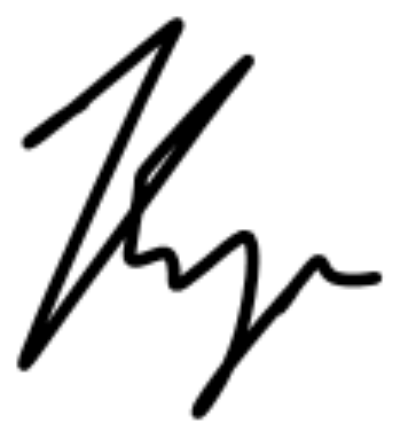
\includegraphics{Graphics/kyen.png} &  \\
     \hline     
     {\bf Kelly Deng} & 1.2. Scope \\ 
      & 2.5. Assumptions and Dependencies\\
      Signature: & 4. Functional Requirements \\
      & \\
      
\includegraphics{Graphics/kelly.jpg} &  \\
      & \\
     \hline
     {\bf Swesan Pathmanathan} & 1.2. Scope \\ 
      & 2.6. Apportioning Requirements \\
      Signature: & 4. Functional Requirements \\
      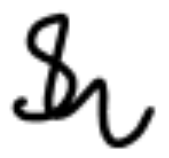
\includegraphics{Graphics/swesan.png} &  \\
     \hline
\end{tabular}
\end{center}
% End Section

%\newpage
%\section*{IMPORTANT NOTES}
%\begin{itemize}
%	\item Be sure to include all sections of the template in your document regardless whether you have something to write for each or not
%	\begin{itemize}
%		\item If you do not have anything to write in a section, indicate this by the \emph{N/A}, \emph{void}, \emph{none}, etc.
%	\end{itemize}
%	\item Uniquely number each of your requirements for easy identification and cross-referencing
%	\item Highlight terms that are defined in Section~1.3 (\textbf{Definitions, Acronyms, and Abbreviations}) with \textbf{bold}, \emph{italic} or \underline{underline}
%	\item For Deliverable 1, please highlight, in some fashion, all (you may have more than one) creative and innovative features. Your creative and innovative features will generally be described in Section~2.2 (\textbf{Product Functions}), but it will depend on the type of creative or innovative features you are including.
%\end{itemize}


\end{document}
%------------------------------------------------------------------------------
